% Well ordering principle question
% Binary search correctness
% Mininum segment tree (recursive correctness)
% Runtime analysis
    % Prove that Big Theta is an equivalence relation (no)
    % Interpolation (no)
% Closed form for recursive functions (no)
% Master theorem
    % Definition
    % Tight asymptotic bound implies regularity
    % Application
% DFA
    % Interpret DFA for strings under length 3 or '100'
    % Create DFA for L((ab + a)*) and prove correctness
    % Prove that the language a^{n^2} is not regular
% Hellish loop correctness (idk yet)
    % Shortest length subarray that has a sum greater than or equal to M
\documentclass{article}
\usepackage{CJKutf8}
\usepackage{amsmath,amssymb,amsthm,enumerate,nicefrac,fancyhdr,hyperref,graphicx,adjustbox,mathtools}
\hypersetup{colorlinks=true,urlcolor=blue,citecolor=blue,linkcolor=blue}
\usepackage[left=3.5cm, right=3.5cm, top=1.5cm, includehead, includefoot]{geometry}
\usepackage[dvipsnames]{xcolor}
\usepackage[d]{esvect}
\usepackage{listings}
\usepackage{enumitem} % To allow for alph in enumerate
\usepackage[normalem]{ulem}
\usepackage{braket}
\usepackage{float} % To allow for H setting in figures.

% to draw dfas
\usepackage{tikz}
\usetikzlibrary{automata, positioning, arrows}

\begin{document}
    \tikzset{
        ->, % makes the edges directed
        >=stealth', % makes the arrow heads bold
        node distance=3cm, % specifies the minimum distance between two nodes. Change if necessary.
        every state/.style={thick, fill=gray!10}, % sets the properties for each ’state’ node
        initial text=$ $, % sets the text that appears on the start arrow
    }
    {\Large NAME (PRINT): \enspace\hrulefill}

    \bigskip

    {\Large STUDENT NUMBER (PRINT): \enspace\hrulefill}

    \bigskip

    \begin{center}
        \fbox{\parbox{\dimexpr\linewidth-2\fboxsep-2\fboxrule\relax}{
            \center
            \textbf{\Large University of Toronto Mississauga} \\

            \textbf{\Large FALL 2024 MOCK FINAL EXAMINATION} \\

            \textbf{\Large Introduction to Theory Computation} \\

            \textbf{\huge M\Large acho \huge M\Large an (m\^{}2)} \\

            \textbf{\Large Duration - \sout{3 hours} 10 minutes} \\

            \textbf{\Large Aids : \begin{CJK}{UTF8}{min}お前のお母さん\end{CJK}} \\
            \smallbreak
        }}
    \end{center}

    This is a mock exam designed for studying CSC236. Any and all similarities with the Fall 2024 CSC236 final examination are purely coincidence.

    If you finish this exam in under 3 hours, you are fully prepared for the final examination.



    \newpage

    \textbf{Q1. (9 points)}
    \smallskip
    Consider the DFA below:
    \begin{center}
        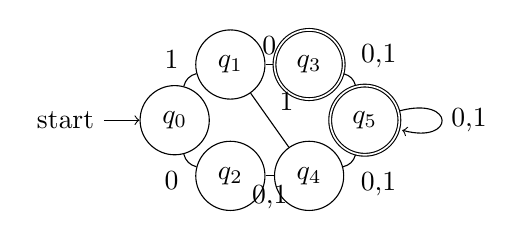
\begin{tikzpicture}
            \node[state, initial] (q0) {\(q_0\)};
            \node[state, above right of=q0] (q1) {\(q_1\)};
            \node[state, below right of=q0] (q2) {\(q_2\)};
            \node[state, accepting, right of=q1] (q3) {\(q_3\)};
            \node[state, right of=q2] (q4) {\(q_4\)};
            \node[state, accepting, below right of=q3] (q5) {\(q_5\)};

            \draw (q0) edge[bend left, above left] node{1} (q1)
                  (q0) edge[bend right, below left] node{0} (q2)
                  (q1) edge[above] node{0} (q3)
                  (q1) edge[above right] node{1} (q4)
                  (q2) edge[below] node{0,1} (q4)
                  (q3) edge[bend left, above right] node{0,1} (q5)
                  (q4) edge[bend right, below right] node{0,1} (q5)
                  (q5) edge[loop right] node{0,1} (q5);
        \end{tikzpicture}
    \end{center}
    \begin{enumerate}[label=\alph*)]
        \item (1 point) Describe the language accepted by the following DFA.

        \item (3 points) Convert this DFA into a minimal NFA (i.e., there is no smaller NFA that accepts this language). Give a brief justification.
        
        \newpage

        \item  (5 points) Provide a DFA that accepts the language matched by \((a+ab)^*\). Prove its correctness.
    \end{enumerate}

    \newpage

    \textbf{Q2. (6 points)}
    \begin{enumerate}[label=\alph*)]
        \item (2 points) State the CLRS version of master theorem. Define all variables and state their conditions.
        \vfill
        \item (2 points) Let \(f: \mathbb{N} \to \mathbb{R}\) be a nonnegative function. Prove that if \(f \in \Theta (n^k)\) for some \(k > 0\), then the regularity condition holds true.
        \vfill
        \item (2 points) Find the time complexity of a recursive function \(T\) defined by
        \[
            T(n) = \begin{dcases}
                4, &\text{ if }  n \leq 1;\\
                3T\left(\frac{n}{2}\right) + n^{2} \log n, &\text{ if } n > 1.
            \end{dcases}
        \]
        \vfill
    \end{enumerate}

    \newpage

    \textbf{Q3. (6 points)}

    \begin{enumerate}[label=\alph*)]
        \item (3 points) Let \(\Sigma = \{0, 1\}\). Let \(L\) be a language on \(\Sigma\) defined by \(L = \{1^{n^2} : n \in \mathbb{N}\}\). Prove that \(L\) is not a regular language.
        \vfill
        \item (3 points) Let \(L, M\) be regular languages. Prove that the language \(L \cap M\) is regular.
        \vfill
    \end{enumerate}

    \newpage

    \textbf{Q4. (6 points)}

    Let \(A\) be a set of functions defined recursively as follows:
    \begin{itemize}
        \item \(\sqrt{x} \in A\) 
        \item If \(f \in A\), then \(\frac{1}{f} - f \in A\) 
    \end{itemize}
    
    \begin{enumerate}[label=\alph*)]
        \item (4 points) Let \(P(f)\) be a predicate on \(A\) and suppose you have managed to prove that
        \begin{itemize}
            \item \(P(\sqrt{x})\) is true,
            \item \(P(f) \implies P(\frac{1}{f} - f)\) for all \(f \in A\).
        \end{itemize}
        Prove that \(\forall f \in A, P(f)\). You may only assume that the principle of induction holds for the natural numbers, NOT the set \(A\).
        \vfill
        \item (2 points) Prove that \(\forall f \in A\), \(f \left( \frac{1}{2} \right) = \frac{1}{\sqrt{2}}\).
        \vfill
    \end{enumerate}

    \newpage

    \textbf{Q5. (7 points)}

    Consider the program below:
    \begin{lstlisting}[language=Python]
    def binary_search(x: int, lst: list[int]):
        l = 0, r = len(lst) - 1
        while(r - l > 0):
            mid = (l+r) // 2
            if(lst[mid] == x):
                return mid
            elif(lst[mid] < x):
                r = mid
            else:
                l = mid + 1
        return l
    \end{lstlisting}
    \begin{enumerate}[label=\alph*)]
        \item (2 points) State the preconditions and postconditions of this program.
        \bigskip
        \item (5 points) Prove that this program is correct.
    \end{enumerate}
    \newpage
\end{document}